%************************************************
\chapter{Results}\label{ch:Results} 
%************************************************
\section{Training cases}
\subsection{Z score threshold}
Investigating the Z score of probes within regions known to be abnormal indicates Z score thresholds that can be applied to mark probes as normal or abnormal (Figure \ref{fig:probeswithinreportedregion}). 
\paragraph*{}
However, reported regions may contain normal probes and whilst sensitivity is favoured over specificity a balance must be found to prevent many false positive calls.

\begin{figure}[h]
\centering
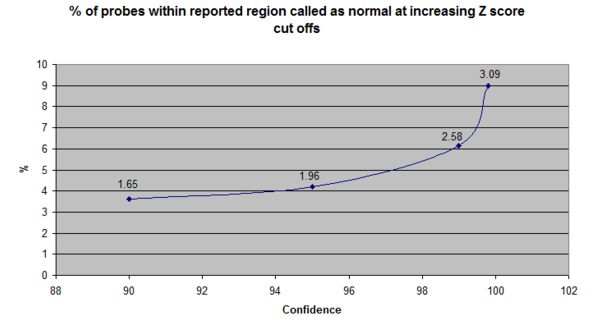
\includegraphics[width=0.9\linewidth]{./Figures/probeswithinreportedregion}
\caption[The number of probes classified as normal within known regions of CNV at a range of Z score thresholds]{The percentage of probes called as normal within known abnormal regions increases with the Z score threshold. Abnormal regions can include normal probes so even at a Z score threshold of 1.65 over 3\% of probes are called as normal. The Z score is shown above each point}
\label{fig:probeswithinreportedregion}
\end{figure}


\subsection{Removal of cases with high false positive calls}
A range of Z score thresholds were applied, starting at $\pm  $ 2.374,  defining abnormal probes as the upper 1\% and lower 1\% of the reference range, and increasing up to $\pm $ 4.25 (Table \ref{tab:training_set_calls_86}).

\begin{table}[h]
\centering
\caption[Calls made in 86 training cases]{A very high number of false positive calls was seen in the 86 training cases using a range of Z score thresholds.}
\label{tab:training_set_calls_86}
\resizebox{\textwidth}{!}{%
\begin{tabular}{@{}lccccccc@{}}
\cmidrule(l){2-8}
\multirow{2}{*}{}                                                                                 & \multicolumn{7}{c}{Z Score}                                                   \\
                                                                                                  & 2.374      & 3         & 3.5      & 3.55     & 3.75     & 4        & 4.25     \\ \cmidrule(l){2-8} 
\% True Positives (n)                                                                             & 92 (79)    & 92 (79)   & 92 (79)  & 92 (79)  & 92 (79)  & 92 (79)  & 88 (76)  \\
\% Arrays with false positives (n)                                                                & 67 (58)    & 45 (39)   & 37 (32)  & 36 (31)  & 33 (28)  & 30 (26)  & 30 (26)  \\
Number of false positive calls                                                                    & 10228        & 7681       & 6177       & 6044       & 5538       & 4944       & 4394       \\
\begin{tabular}[c]{@{}l@{}}Average number of false \\ positive calls per array (max)\end{tabular} & 192.98 (2128) & 225.91 (1733) & 228.78 (1468) & 232.46 (1443) & 240.78 (1351) & 235.43 (1230) & 209.24 (1108)
\end{tabular}%
}
\end{table}

\paragraph*{}
At the lowest Z score threshold (2.374) the false negative rate was 8\% with 67\% of cases containing a false positive call.
\paragraph*{}
The same Z score threshold resulted in 10228 false positive calls, of which 94\% came from just five arrays (range 1612-2128). The average number of false positive calls in the other 81 arrays was 10.8 (max 104) (Table \ref{tab:training_set_calls}).
\paragraph*{}
Visual inspection of the array traces and the raw data from these 5 arrays gave no indication why so many false positives calls were made or how this could be predicted. Therefore these five arrays were considered a different population and excluded from further analysis.
\subsection{Comparison of true positive and false positive calls}
\begin{table}[]
\centering
\caption[Calls made in 81 training cases after removal of outliers]{The calls made in 81 training cases using a range of Z score thresholds. The true positive call was missed in at least 5 cases across all thresholds, with a false positive call made in at least 1 in 4 cases. The number of false positive calls, and the average number of calls made decreased as the Z score threshold increased.}
\label{tab:training_set_calls}
\resizebox{\textwidth}{!}{%
\begin{tabular}{@{}lccccccc@{}}
\cmidrule(l){2-8}
\multirow{2}{*}{}                                                                                 & \multicolumn{7}{c}{Z Score}                                                   \\
                                                                                                  & 2.374      & 3         & 3.5      & 3.55     & 3.75     & 4        & 4.25     \\ \cmidrule(l){2-8} 
\% True Positives (n)                                                                             & 94 (76)    & 94 (76)   & 94 (76)  & 94 (76)  & 94 (76)  & 94 (76)  & 90 (73)  \\
\% Arrays with false positives (n)                                                                & 65 (53)    & 42 (34)   & 33 (27)  & 32 (26)  & 28 (23)  & 26 (21)  & 26 (21)  \\
Number of false positive calls                                                                    & 571        & 114       & 50       & 48       & 41       & 35       & 31       \\
\begin{tabular}[c]{@{}l@{}}Average number of false \\ positive calls per array (max)\end{tabular} & 10.8 (104) & 3.35 (20) & 1.85 (7) & 1.84 (7) & 1.78 (7) & 1.66 (6) & 1.48 (5)
\end{tabular}%
}
\end{table}
The remaining 81 arrays show that at least one call was detected within the abnormal region in 94\% of cases with a Z score up to 4 (Table \ref{tab:training_set_calls}).
\\
Using a Z score of 2.374 nearly 2 in 3 arrays had a false positive call. A Z score threshold of 4 reduced the frequency of false positive calls to 1 in 4 arrays, with an average 1.66 and maximum 6 false positive calls per array.

\subsubsection{Number of probes within a call}
The length of false positive calls are shorter than true positive calls. Increasing the minimum number of probes within a call would remove these false positive calls but would also remove true positive calls and fail to meet the functional requirement that a call is a minimum of 3 consecutive probes (Figure \ref{fig:nprobes_2_374}).

\begin{figure}[h]
\centering
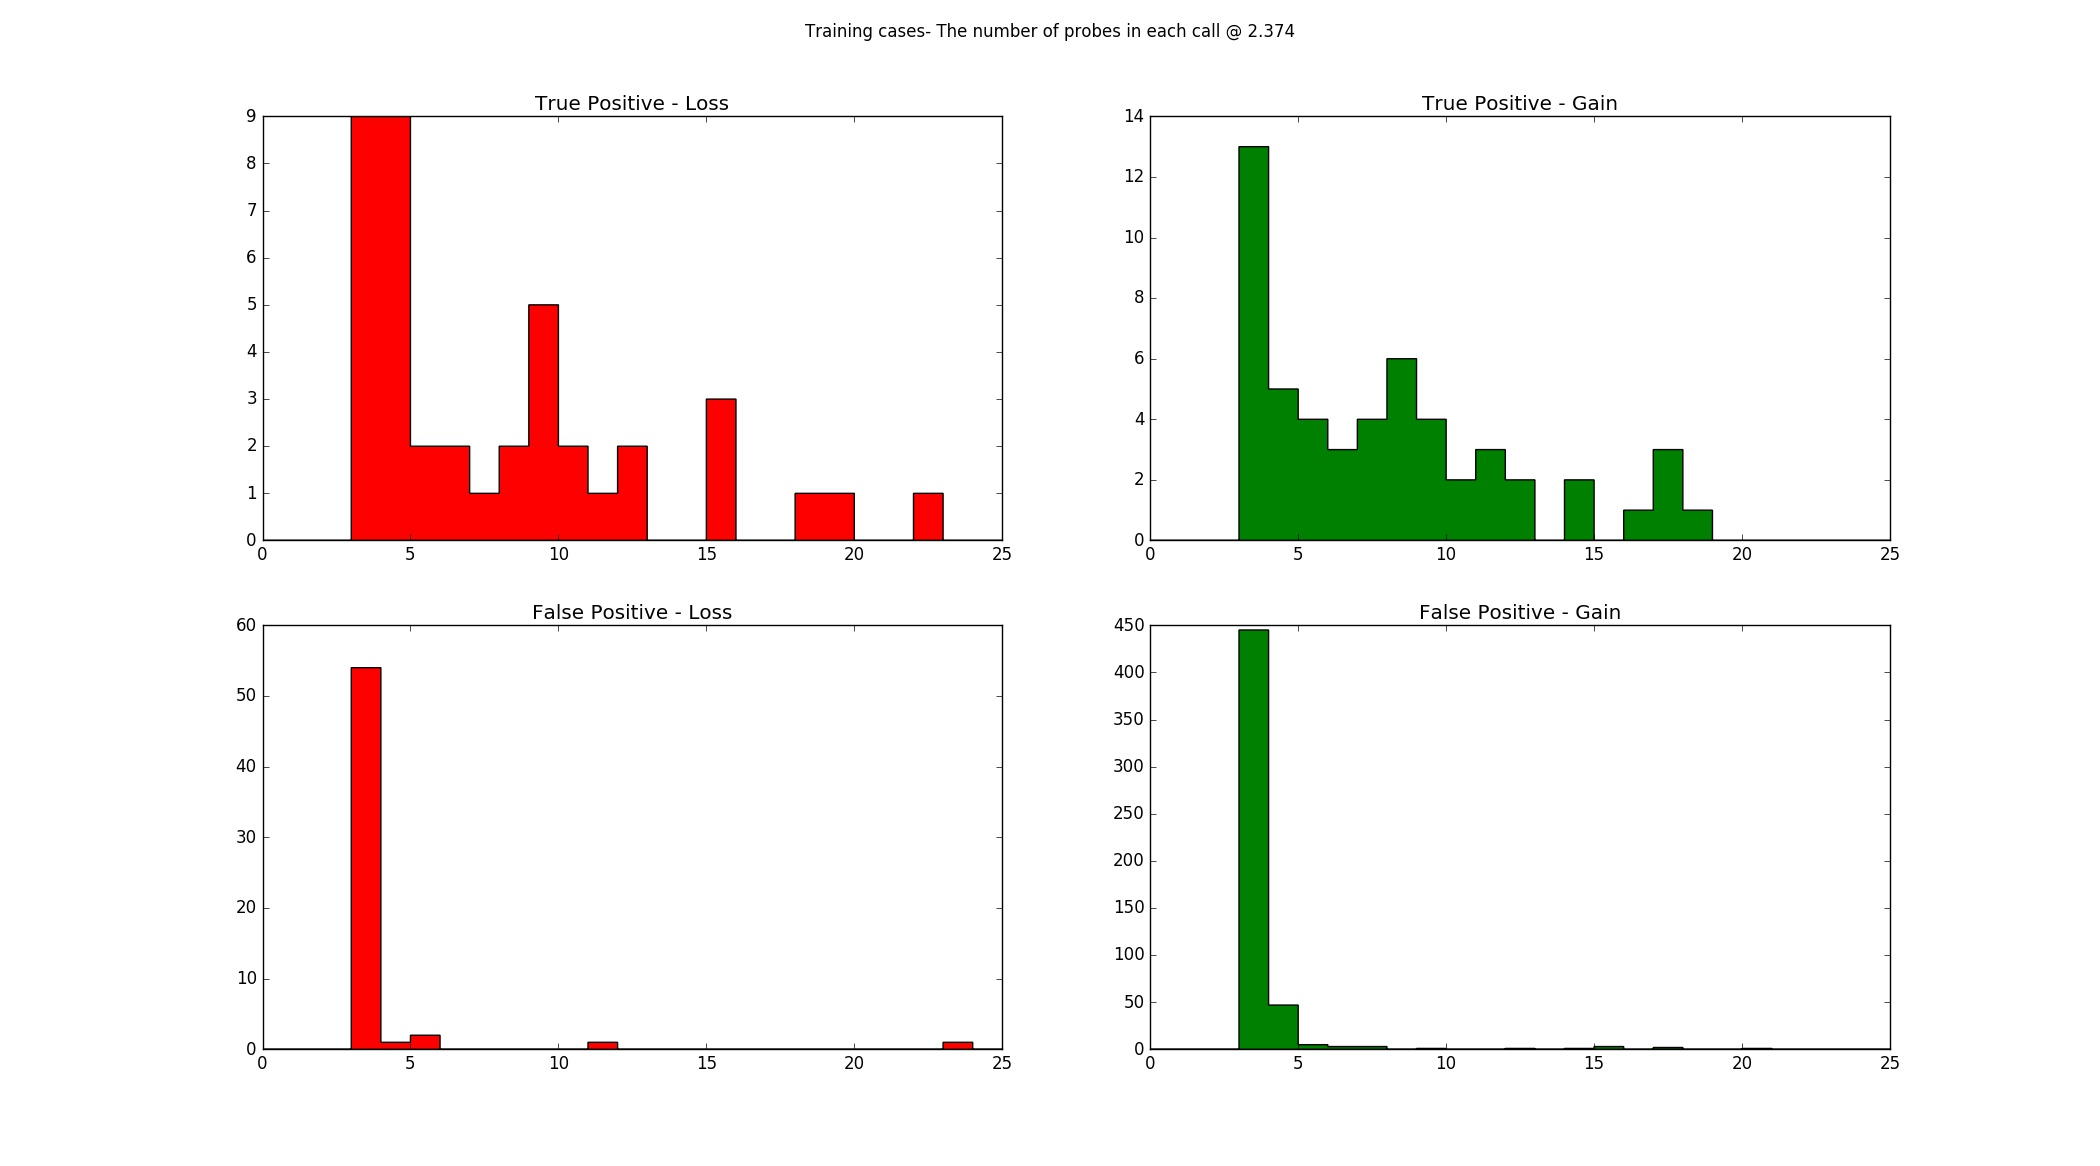
\includegraphics[width=\linewidth]{./Figures/nprobes_2_374}
\caption{Training cases: False positive calls are smaller than true positive calls.}
\label{fig:nprobes_2_374}
\end{figure}

\subsubsection{Difference between true and false positive Z scores using a threshold of 2.374}
Alternatively increasing the Z score threshold to above the lowest scoring probe in abnormal regions may prevent the region being called (Figure \ref{fig:consecutiveprobeanalysis}).
\paragraph*{}
Examining the minimum (Figure \ref{fig:lowest_2_374}) and average (Figure \ref{fig:average_2_374}) Z scores for each true and false positive calls show that the two populations are not disparate therefore increasing the Z score threshold may also remove true positives. 
\begin{figure}[h]
\centering
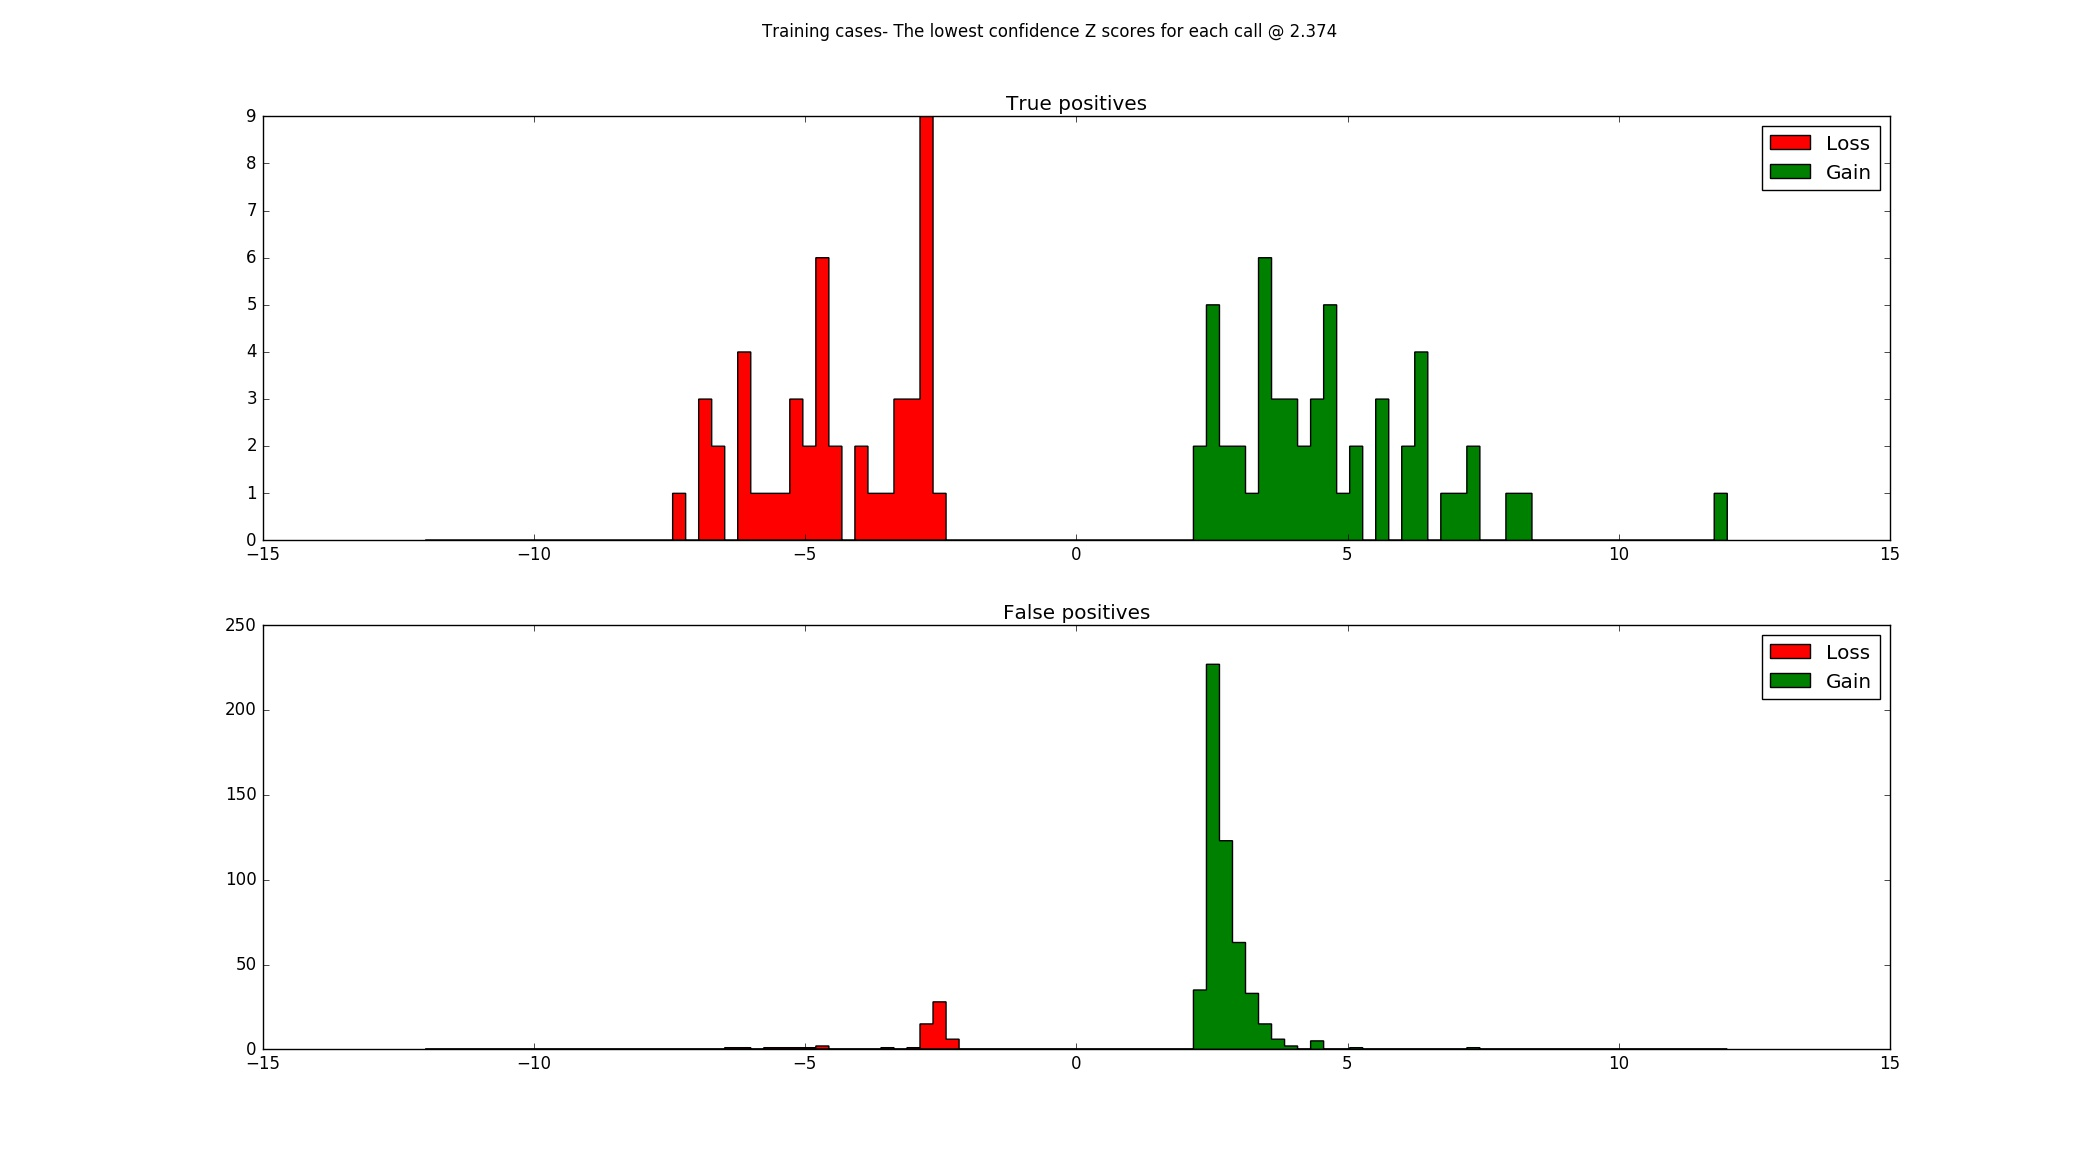
\includegraphics[width=1\linewidth]{./Figures/lowest_2_374}
\caption[Training cases: The lowest confidence Z score within each call at a threshold of 2.374]{Training cases: The lowest confidence Z score within each call at a threshold of 2.374. There is an overlap between the confidence of the lowest probe within true and false positive calls}
\label{fig:lowest_2_374}
\end{figure}

\begin{figure}[h]
\centering
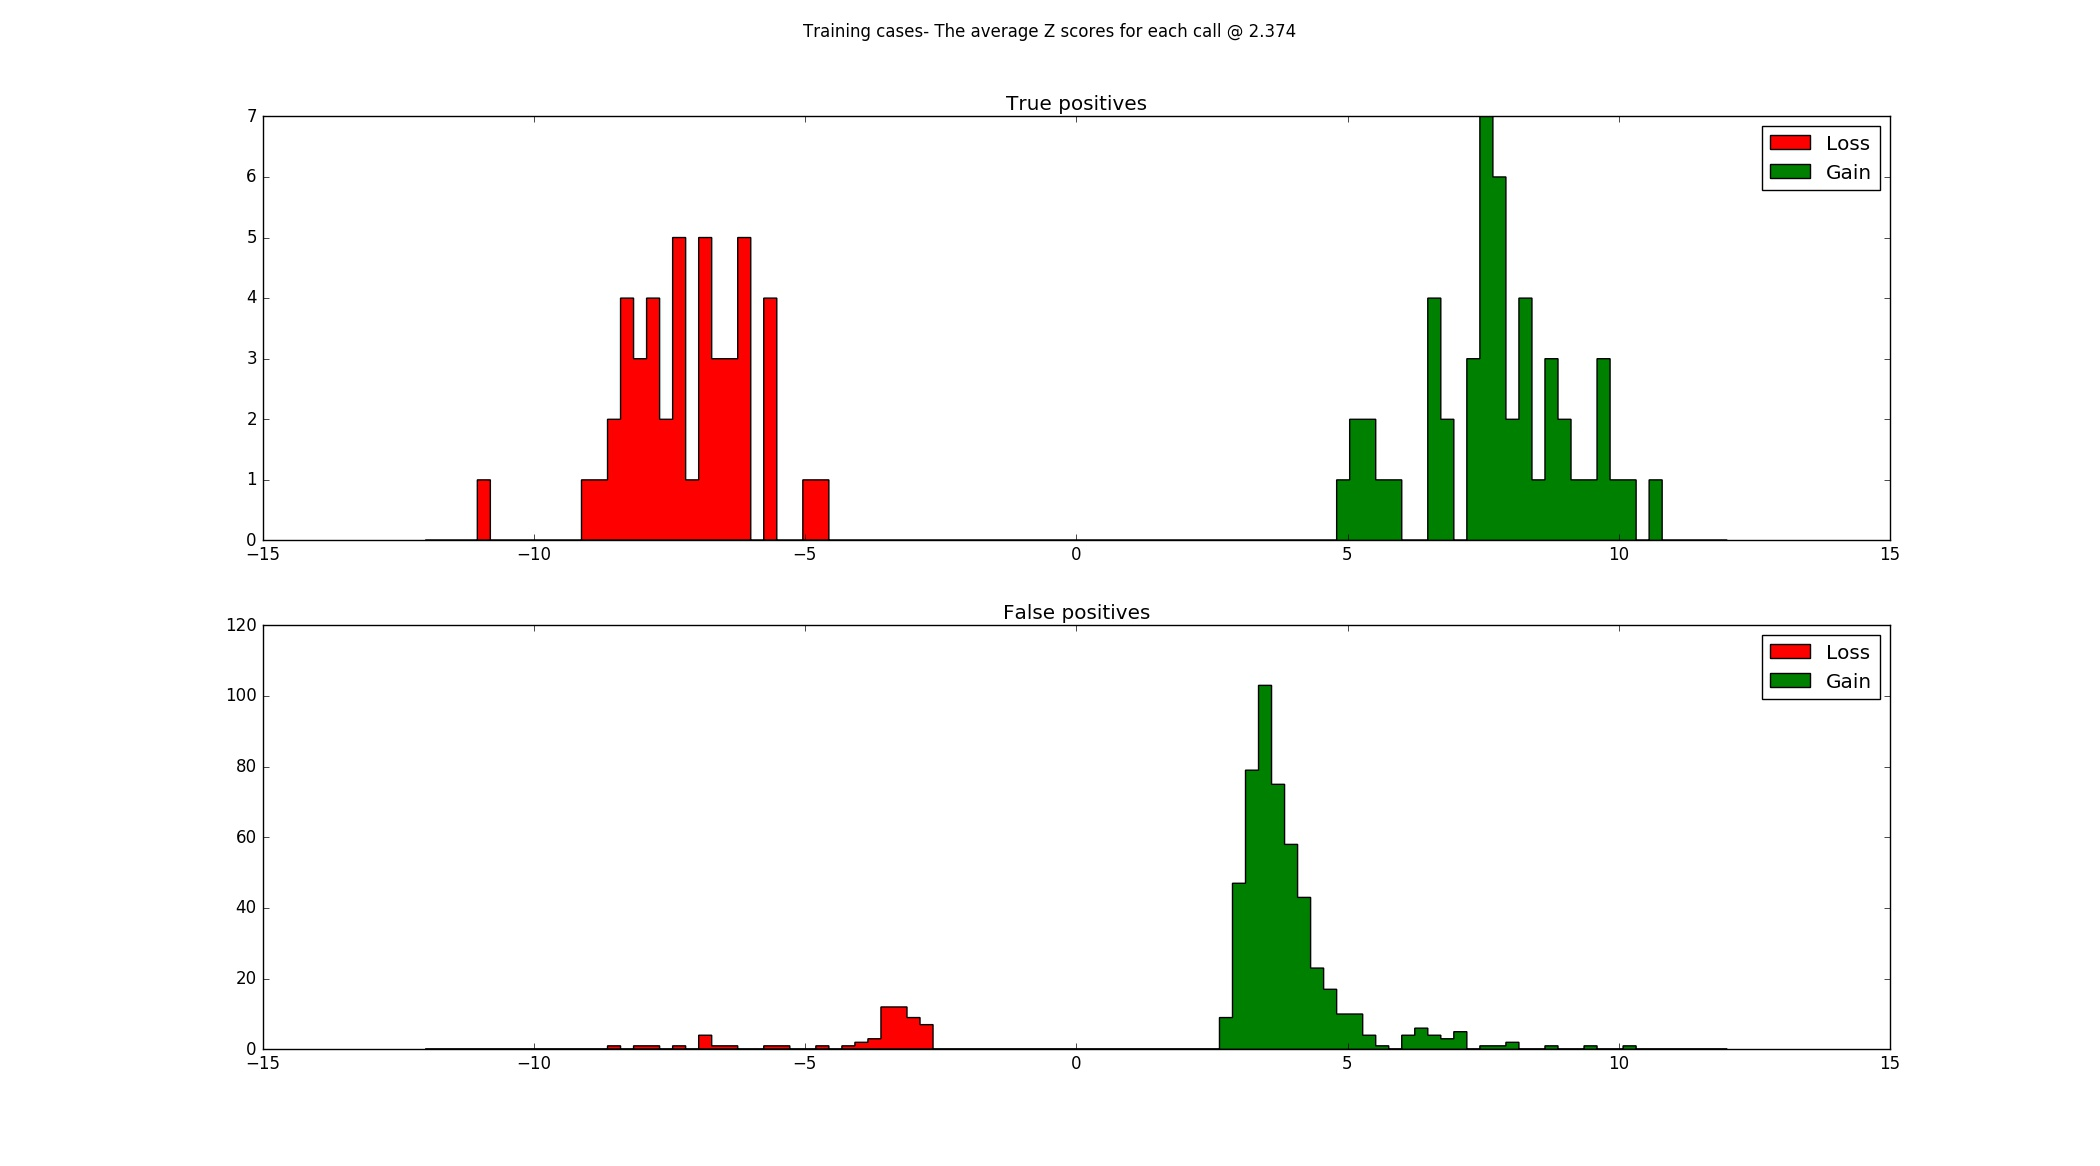
\includegraphics[width=1\linewidth]{./Figures/average_2_374}
\caption[Training cases: The average Z score of probes within calls at a threshold of 2.374]{Training cases: The average Z score of probes within calls at a threshold of 2.374. The average Z score of true positive calls are further from the mean than the average Z score of false positive calls.}
\label{fig:average_2_374}
\end{figure}

\paragraph*{}
However the increased number of probes within a true positive region (Figure \ref{fig:nprobes_2_374}) and the higher average Z score (Figure \ref{fig:average_2_374}) may mean the true positive regions remain.

\subsubsection{Difference between true and false positive Z scores using a threshold of 3.55}
Increasing the Z score threshold to 3.55 showed that the average and lowest confidence Z scores in remaining false positive calls were similar to that of true positives (Figures \ref{fig:lowest_3_55} and \ref{fig:average_3_55}).

\begin{figure}[h]
\centering
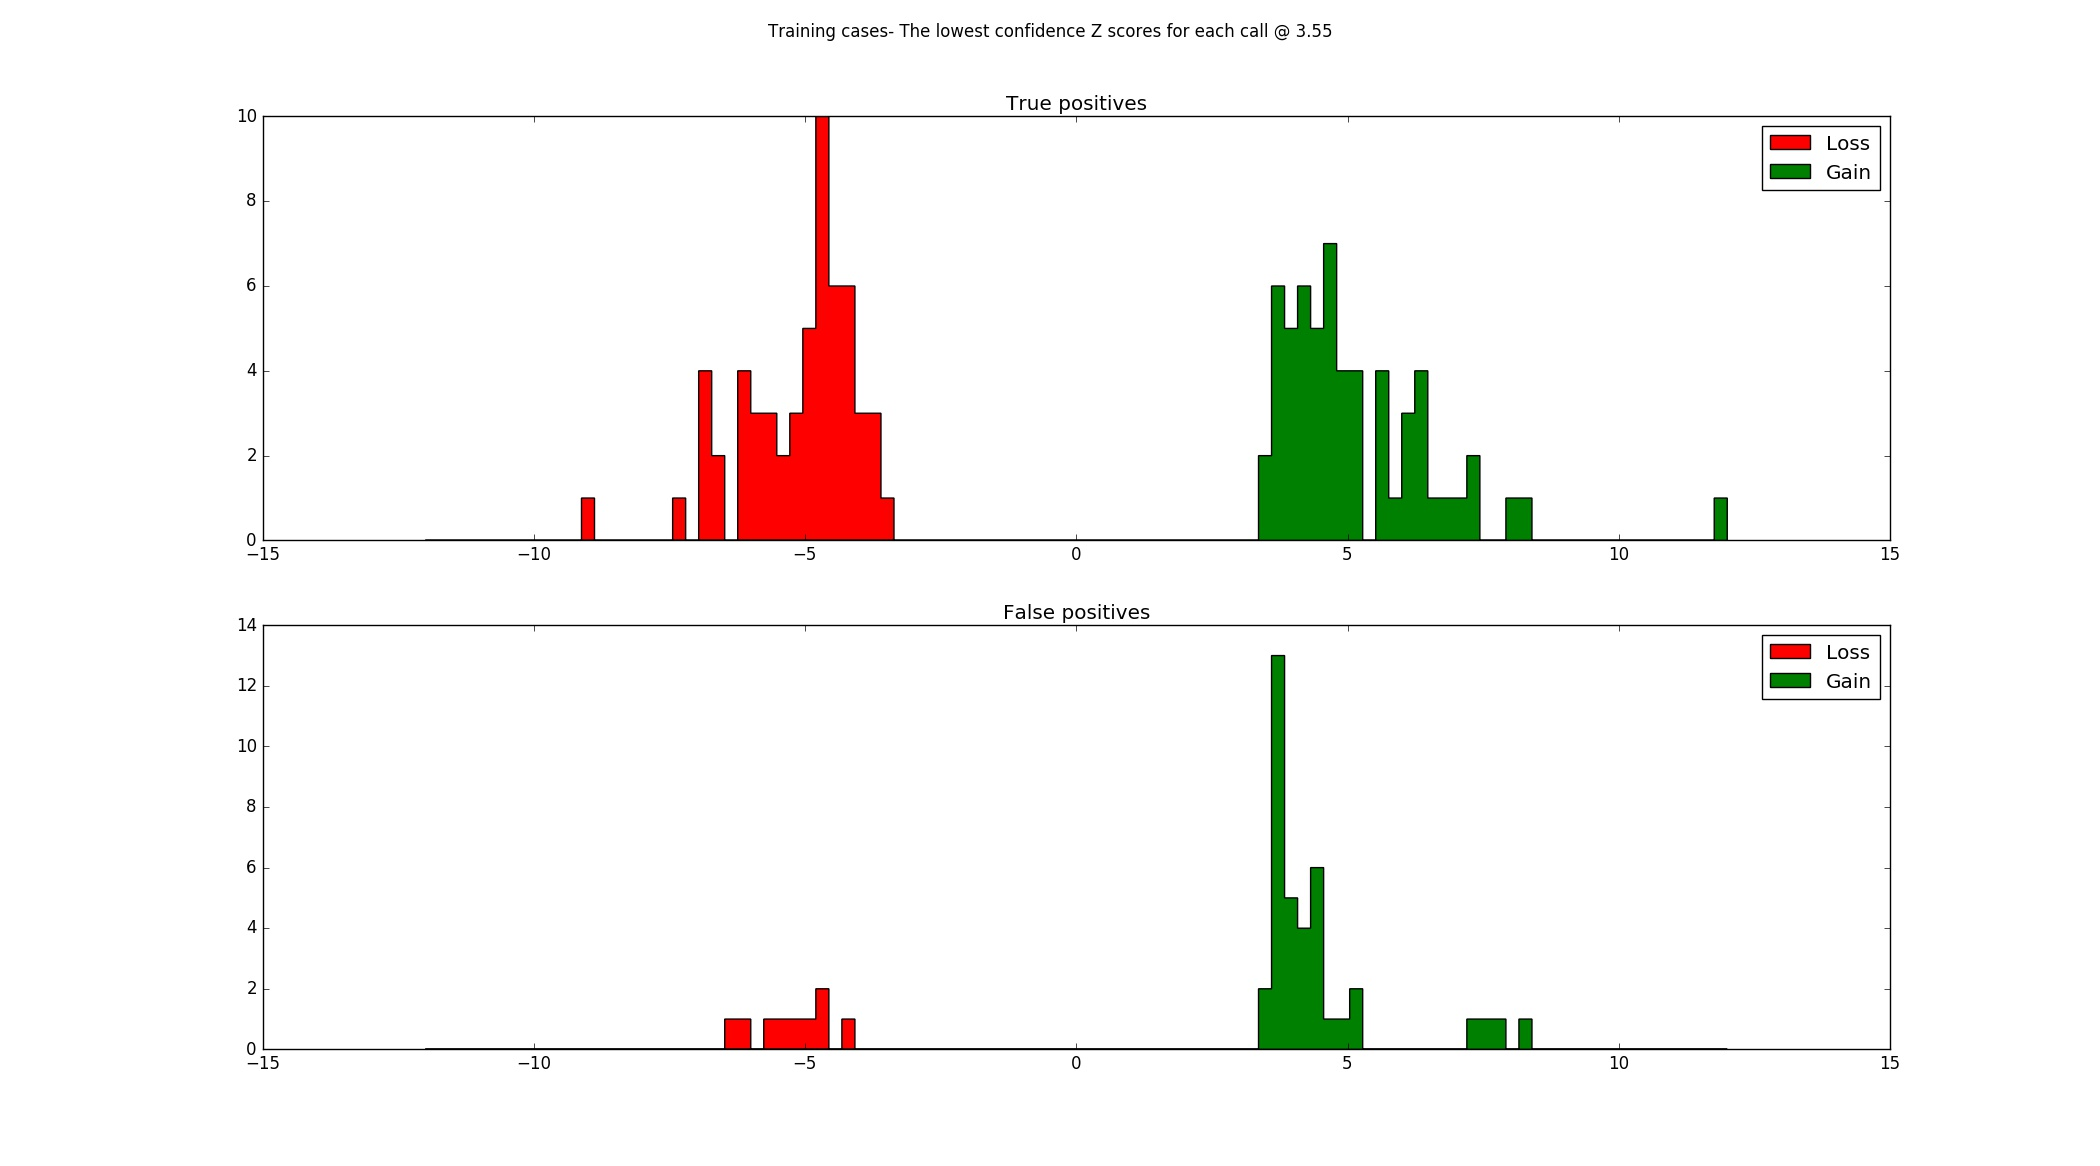
\includegraphics[width=1\linewidth]{./Figures/lowest_3_55}
\caption[Training cases: The lowest confidence probe within calls at a threshold of 3.55]{Training cases: At a threshold of 3.55 the lowest confidence probes within true and false calls are very similar}
\label{fig:lowest_3_55}
\end{figure}

\begin{figure}[h]
\centering
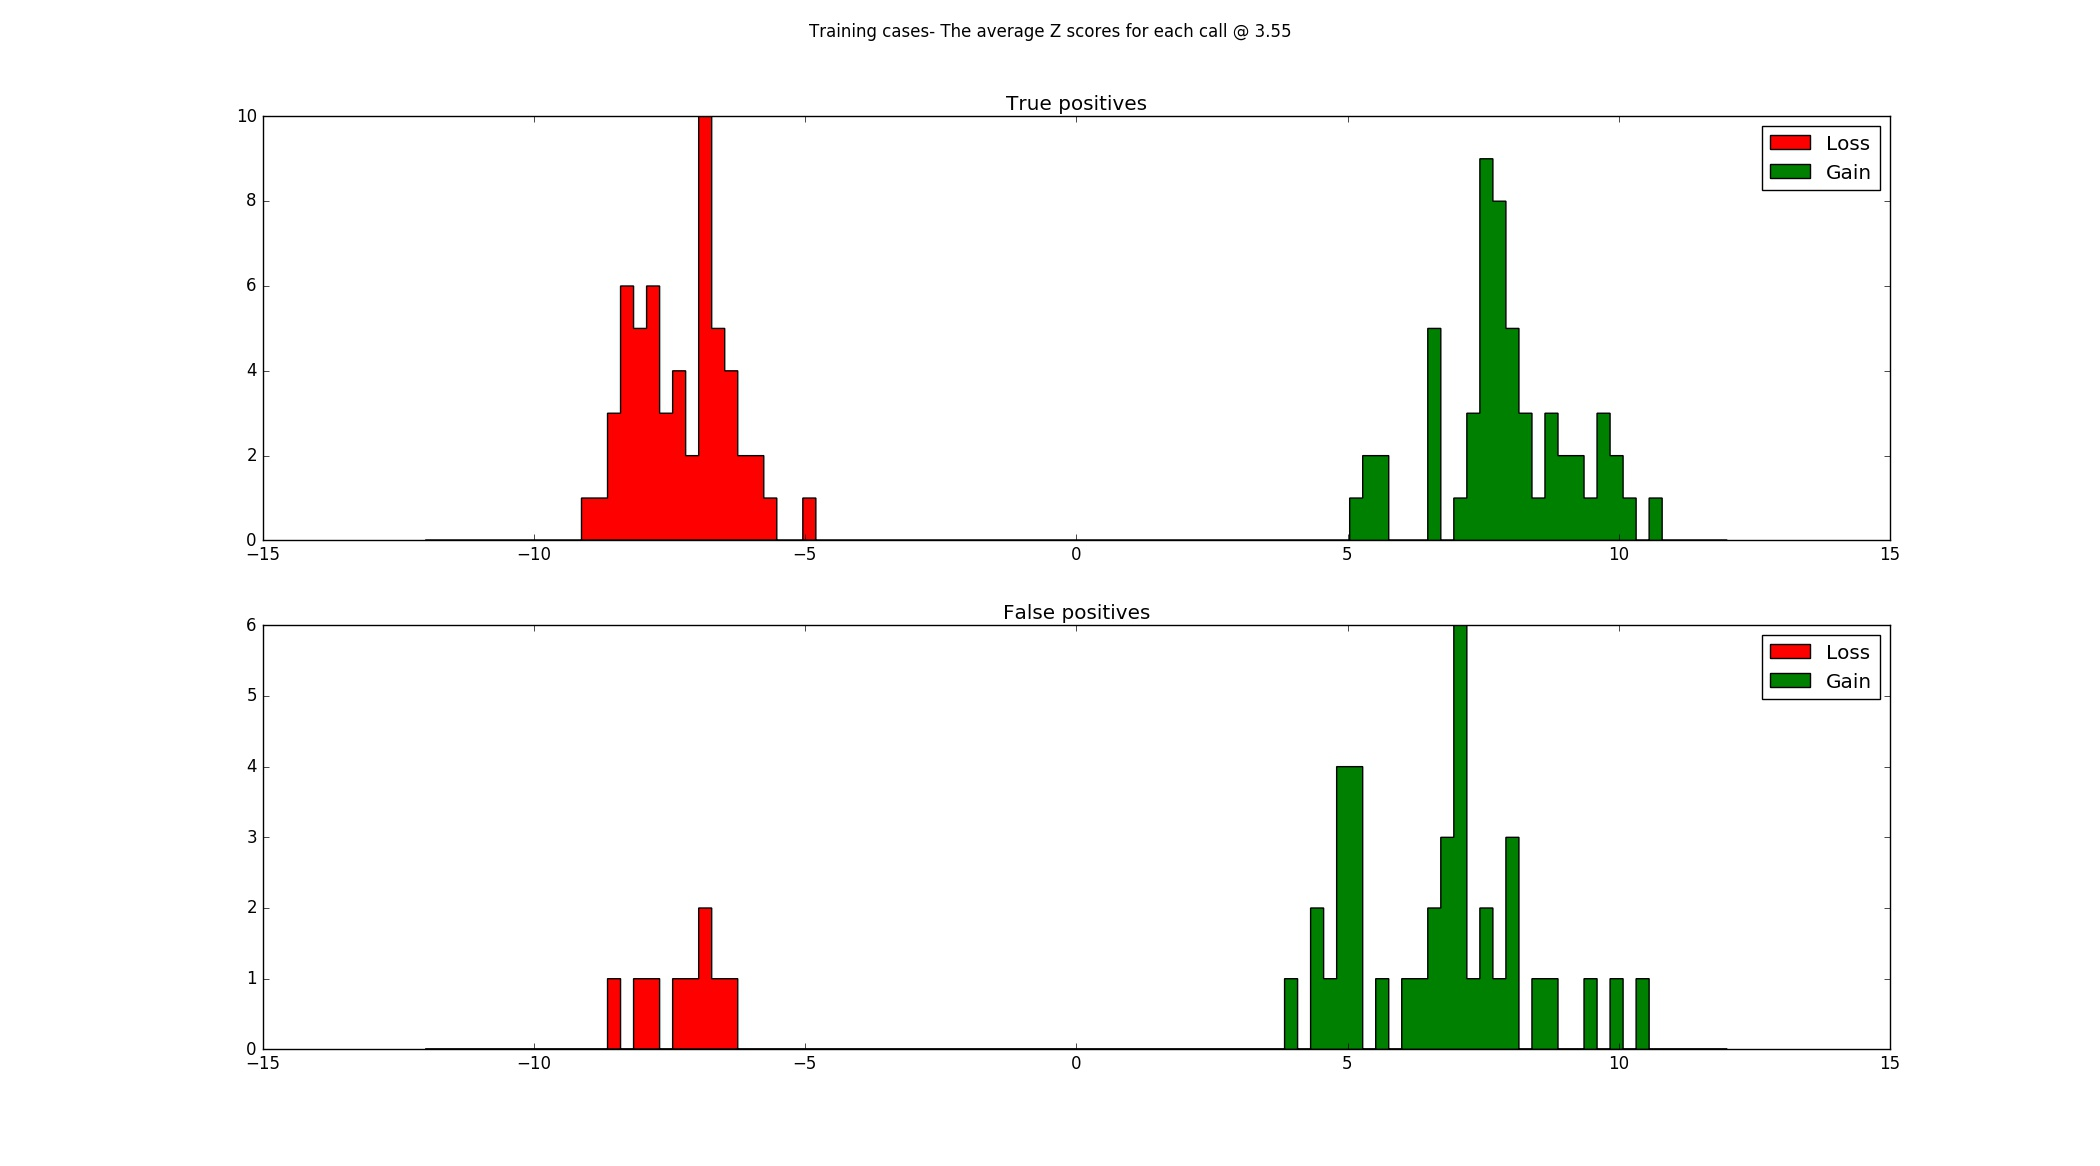
\includegraphics[width=1\linewidth]{./Figures/average_3_55}
\caption[Training cases:Average Z scores for calls made with a threshold of 3.55]{Training cases: The average Z score for probes within true and false positive calls with a threshold of 3.55 are very similar.}
\label{fig:average_3_55}
\end{figure}

\subsubsection{Suitability of reference range}
There were no recurring false positives calls to suggest the reference range is unsuitable.